% What is coming with group work: orienting the class before groups form.
% Shared preamble for the write-on class slides.
%
% Every deck is designed to be projected and annotated live on a tablet:
% whatever takes time to draw is pre-drawn, and whatever the class produces is
% left blank. Compile a deck with `pdflatex main.tex` from its own directory,
% or run `uv run python build.py` from the repository root to build them all.
\documentclass[10pt]{article}

\usepackage[papersize={25.6cm,14.4cm}, margin=1.1cm, bottom=1.5cm,
            footskip=0.75cm]{geometry}
\usepackage[T1]{fontenc}
\usepackage[default]{sourcesanspro}
\usepackage{newtxsf}
\usepackage{tikz}
\usepackage{amsmath}
\usepackage{parskip}
\usepackage{fancyhdr}
\usetikzlibrary{arrows.meta, positioning, calc}

\setlength{\parindent}{0pt}

% Catppuccin Latte, the palette the course site uses in its light theme, so a
% deck on the projector looks like the pages the students read.
\definecolor{inkbg}{HTML}{EFF1F5}      % base
\definecolor{inksurface}{HTML}{E6E9EF} % mantle
\definecolor{inkfaint}{HTML}{CCD0DA}   % surface2, for rules and empty boxes
\definecolor{inktext}{HTML}{4C4F69}    % text
\definecolor{inkgrey}{HTML}{8C8FA1}    % overlay1, for anything secondary
\definecolor{inkblue}{HTML}{7287FD}    % lavender, the primary accent
\definecolor{inkteal}{HTML}{179299}    % teal
\definecolor{inkred}{HTML}{FE640B}     % peach, for whatever wants attention
\definecolor{inkmauve}{HTML}{8839EF}   % mauve

\pagecolor{inkbg}
\color{inktext}

% A box to write a short answer into. White against the tinted page, so it
% reads as somewhere to write rather than as part of the printed material.
\newcommand{\blank}[1][1.6]{%
  \tikz[baseline=(current bounding box.base)]{%
    \draw[inkfaint, line width=0.7pt, rounded corners=2pt, fill=white]
      (0,-0.18) rectangle (#1,0.62);}}

% A ruled area to work in. Faint dots keep handwriting level on a tablet.
\newcommand{\workspace}[2]{%
  \begin{tikzpicture}
    \draw[inkfaint, line width=0.7pt, rounded corners=3pt, fill=white]
      (0,0) rectangle (#1,#2);
    \foreach \gx in {0.5,1.0,...,#1}{%
      \foreach \gy in {0.5,1.0,...,#2}{%
        \fill[inkfaint] (\gx,\gy) circle (0.5pt);}}
  \end{tikzpicture}}

% A panel for material that is printed rather than written on.
\newcommand{\panel}[2]{%
  \begin{tikzpicture}
    \draw[inkfaint, line width=0.7pt, rounded corners=3pt, fill=inksurface]
      (0,0) rectangle (#1,#2);
  \end{tikzpicture}}

% A labelled card of printed material. #2 and #3 are widths in cm; the text
% column is the card less its padding, computed rather than guessed.
\newcommand{\cardbox}[4]{%
  \begin{tikzpicture}
    \node[draw=#1, line width=1pt, rounded corners=4pt, fill=white,
          minimum width=#2cm, minimum height=#3cm,
          text width=\dimexpr#2cm-0.9cm\relax,
          align=left, inner sep=0.45cm, text=inktext] {#4};
  \end{tikzpicture}}

% A card whose body is left blank for the class to fill in.
\newcommand{\cardblank}[4]{%
  \begin{tikzpicture}
    \node[draw=#1, line width=1pt, rounded corners=4pt, fill=white,
          minimum width=#2cm, minimum height=#3cm,
          text width=\dimexpr#2cm-0.9cm\relax,
          align=left, inner sep=0.45cm, text=inktext, anchor=north west]
      at (0,0) {#4};
  \end{tikzpicture}}

% Running header: the deck name on the left, the page's own step on the right.
% Each deck sets its name once with \deckname.
\newcommand{\deck}{}
\newcommand{\deckname}[1]{\renewcommand{\deck}{#1}}
\newcommand{\slidehead}[1]{%
  {\small\color{inkgrey}%
   \tikz[baseline=-0.5ex]{\fill[inkblue, rounded corners=1pt]
     (0,0) rectangle (0.22,0.22);}\;\deck
   \hfill \color{inkblue}\bfseries #1}\par
  {\color{inkblue}\rule{\linewidth}{1pt}}\par\vspace{0.35em}}

\pagestyle{fancy}
\fancyhf{}
\renewcommand{\headrulewidth}{0pt}
\fancyfoot[R]{\small\color{inkgrey}\thepage}

% Deck title pages, which carry no header and no page number.
\newcommand{\titleslide}[3]{%
  \thispagestyle{empty}%
  \begin{center}
    \vspace*{\fill}
    {\Huge\bfseries\color{inkblue} #1}\\[0.7em]
    {\LARGE\color{inkgrey} #2}\\[2.4em]
    #3
    \vspace*{\fill}
  \end{center}}

% One step of the plan on a title page.
\newcommand{\stepbox}[3]{%
  \node[draw=inkblue, line width=0.9pt, rounded corners=4pt, fill=white,
        minimum width=6cm, minimum height=1.7cm, align=center,
        text=inktext] (#1) at (#2,0) {#3};}

% Prompt to the room: a question the class answers, not something I read out.
\newcommand{\ask}[1]{%
  {\large\color{inkblue}\bfseries #1}\par\vspace{0.5em}}


\deckname{What is coming with group work}

\begin{document}

\titleslide{What is coming with group work}{The group project, in twenty minutes}{%
    
\begin{tikzpicture}[font=\small]
      \stepbox{s0}{0.0}{\textbf{Build}\\[0.25em] A library, in a four.}
      \stepbox{s1}{6.9}{\textbf{Marked}\\[0.25em] On you \emph{and} on the group.}
      \stepbox{s2}{13.8}{\textbf{Now}\\[0.25em] Form your group.}
      \draw[-{Stealth[length=2.5mm]}, inkfaint, line width=1.2pt] (s0) -- (s1);
      \draw[-{Stealth[length=2.5mm]}, inkfaint, line width=1.2pt] (s1) -- (s2);
    \end{tikzpicture}}

\newpage
\slidehead{Before I say anything}

\vfill

\begin{center}
{\fontsize{120}{130}\selectfont\bfseries\color{inkblue} Group work}
\end{center}

\vfill

\newpage
\slidehead{The shape of it}

\vspace{1.2cm}

\begin{center}
{\Huge\bfseries\color{inkblue} 60\%} \qquad
{\LARGE\color{inktext} of your mark} \qquad
{\LARGE\color{inkgrey} from} \qquad
{\Huge\bfseries\color{inkblue} Week 4}
\end{center}

\vspace{1.4cm}

\begin{center}
{\LARGE A \textbf{Python library} for a mathematical problem of your choice,
built in a group of \textbf{four}.}
\end{center}

\vspace{1.0cm}

\begin{center}
{\large\color{inkgrey} Of your choice, and you do not have to choose it
alone. Come and talk to me about it.}
\end{center}

\newpage
\slidehead{What you hand in}

\vspace{0.7cm}

\begin{center}
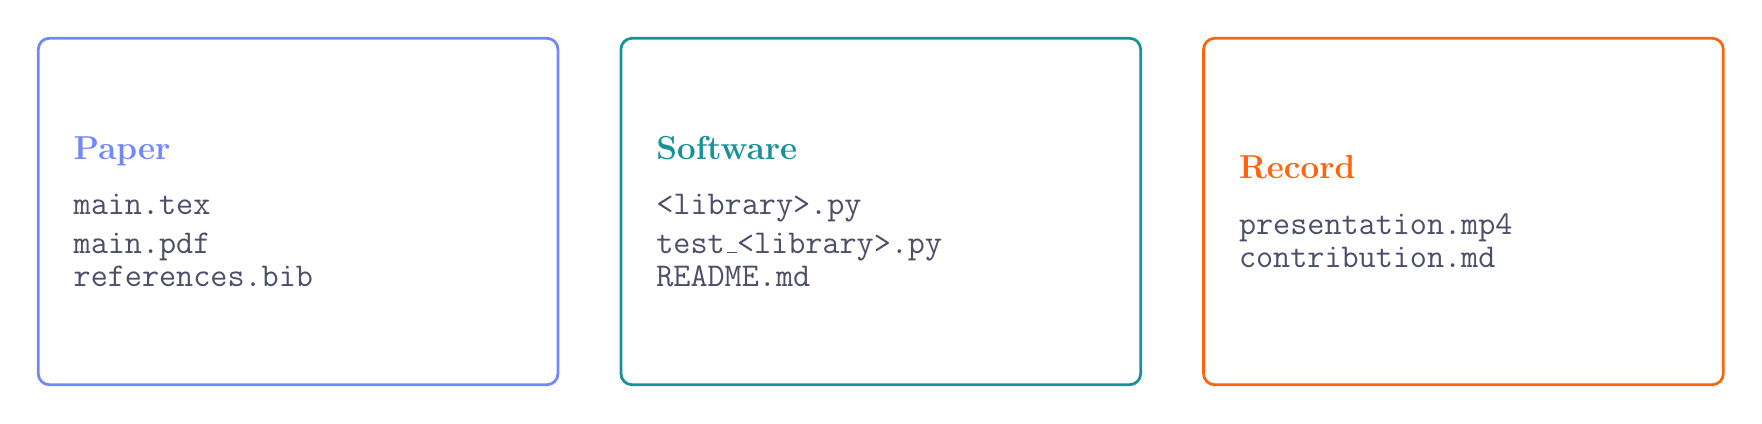
\begin{tikzpicture}
  \node (a) at (0,0) {\cardbox{inkblue}{6.6}{4.4}{%
    {\large\bfseries\color{inkblue} Paper}\\[0.6em]
    {\large\ttfamily main.tex\\ main.pdf\\ references.bib}}};
  \node (b) at (7.4,0) {\cardbox{inkteal}{6.6}{4.4}{%
    {\large\bfseries\color{inkteal} Software}\\[0.6em]
    {\large\ttfamily <library>.py\\ test\_<library>.py\\ README.md}}};
  \node (c) at (14.8,0) {\cardbox{inkred}{6.6}{4.4}{%
    {\large\bfseries\color{inkred} Record}\\[0.6em]
    {\large\ttfamily presentation.mp4\\ contribution.md}}};
\end{tikzpicture}
\end{center}

\vspace{0.9cm}

\begin{center}
{\LARGE All \;\blank[2.4]\; of them are graded.}
\end{center}

\newpage
\slidehead{How your mark is worked out}

\vspace{0.7cm}

\begin{center}
{\Huge \(\text{Final mark} = \sqrt{I \times Q}\)}
\end{center}

\vspace{0.9cm}

\begin{center}

\begin{tikzpicture}
  \node at (0,0) {\cardbox{inkblue}{10.2}{4.4}{%
    {\Large\bfseries\color{inkblue} \(I\)}}};
  \node at (11.8,0) {\cardbox{inkteal}{10.2}{4.4}{%
    {\Large\bfseries\color{inkteal} \(Q\)}}};
\end{tikzpicture}
\end{center}

\vspace{0.7cm}

\ask{What goes in each one?}

\newpage
\slidehead{A strong group}

\vspace{0.4cm}

\begin{minipage}[c]{0.40\linewidth}
\begin{center}
{\color{inkgrey}\LARGE The group's mark}

\vspace{0.5em}

{\fontsize{72}{78}\selectfont\bfseries\color{inkteal} \(Q = 74\)}

\vspace{1.2em}

{\LARGE\color{inktext} \(\sqrt{I \times Q}\)}
\end{center}
\end{minipage}
\hfill
\begin{minipage}[c]{0.56\linewidth}
\begin{center}
{\LARGE
\begin{tabular}{llc}
  \textbf{Student} & \(I\) & \textbf{Final mark}\\[0.4em]
  \hline
  \rule{0pt}{1.5em}A & 100 & \blank[3.2]\\[0.7em]
  B & 80 & \blank[3.2]\\[0.7em]
  C & 80 & \blank[3.2]\\[0.7em]
  \color{inkred}D & \color{inkred}20 & \blank[3.2]\\
\end{tabular}}
\end{center}
\end{minipage}

\vspace{0.6cm}

\ask{The group did well. What happens to D?}

\newpage
\slidehead{So where does \(I\) come from?}

\vspace{0.7cm}

\begin{center}
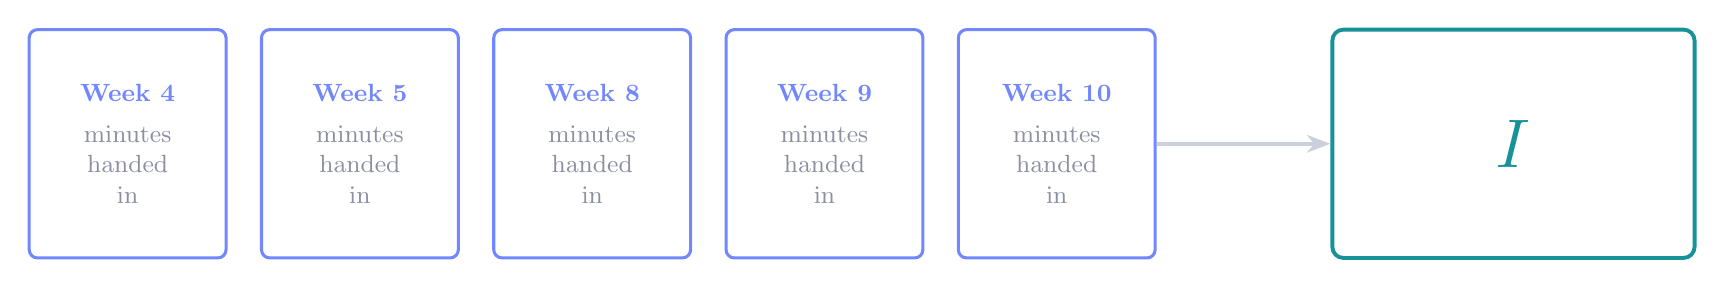
\begin{tikzpicture}
  \foreach \w [count=\n from 0] in {4, 5, 8, 9, 10}{%
    \node[draw=inkblue, line width=1.1pt, rounded corners=3pt, fill=white,
          minimum width=2.5cm, minimum height=2.9cm, align=center,
          font=\small, text=inkgrey] (f\n) at (\n*2.95,0)
      {\textbf{\color{inkblue} Week \w}\\[0.4em] minutes\\ handed\\ in};}
  \node[draw=inkteal, line width=1.4pt, rounded corners=4pt, fill=white,
        minimum width=4.6cm, minimum height=2.9cm, align=center,
        font=\large, text=inktext] (i) at (17.6,0)
    {{\Huge\bfseries\color{inkteal} \(I\)}};
  \draw[-{Stealth[length=3mm]}, inkfaint, line width=1.4pt]
    (f4.east) -- (i.west);
\end{tikzpicture}
\end{center}

\vspace{0.8cm}

\begin{center}
{\LARGE Your group hands in \textbf{one form, every group-project week}.\\[0.5em]
 It is the \textbf{only} record of who engaged.}
\end{center}

\vspace{0.6cm}

\begin{center}
{\large Recorded as engaged at 3 of the 5?\quad
 \(I = {}\)\;\blank[2.6]}
\end{center}

\newpage
\slidehead{Who teaches you these chapters?}

\vspace{0.5cm}

\begin{center}
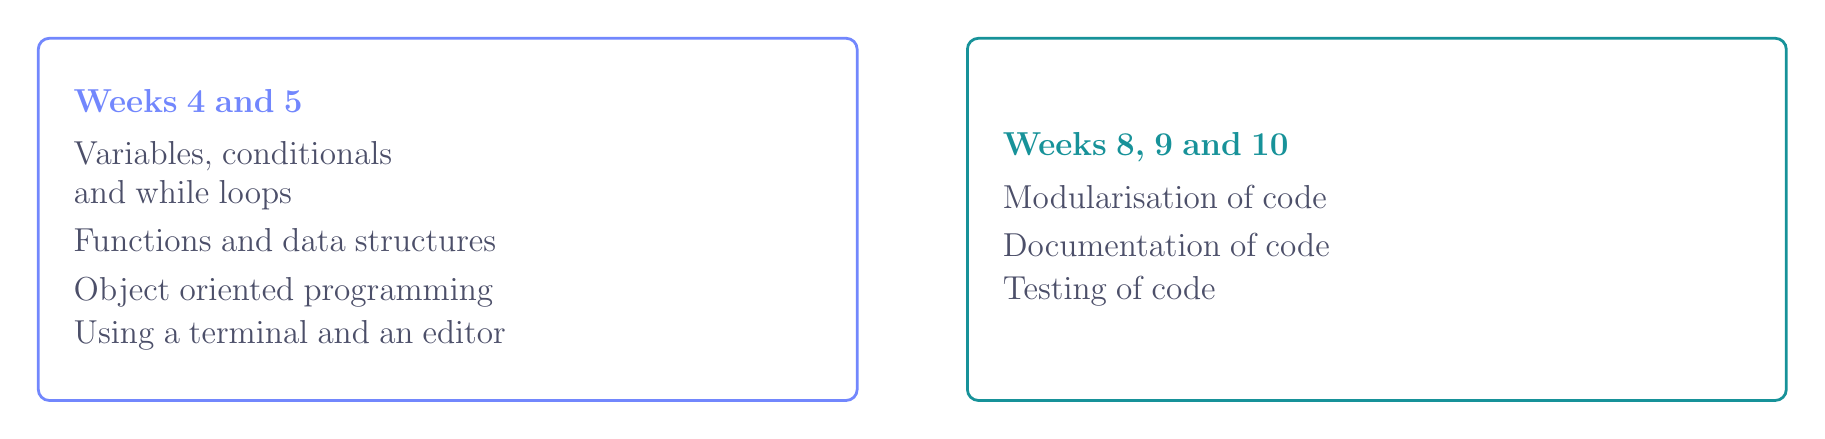
\begin{tikzpicture}
  \node at (0,0) {\cardbox{inkblue}{10.4}{4.6}{%
    {\large\bfseries\color{inkblue} Weeks 4 and 5}\\[0.5em]
    {\large Variables, conditionals\\ and while loops\\[0.3em]
     Functions and data structures\\[0.3em]
     Object oriented programming\\[0.3em]
     Using a terminal and an editor}}};
  \node at (11.8,0) {\cardbox{inkteal}{10.4}{4.6}{%
    {\large\bfseries\color{inkteal} Weeks 8, 9 and 10}\\[0.5em]
    {\large Modularisation of code\\[0.3em]
     Documentation of code\\[0.3em]
     Testing of code}}};
\end{tikzpicture}
\end{center}

\vspace{0.7cm}

\ask{There is no lecture on any of these. So who teaches them to you?}

\newpage
\slidehead{Yes: this is self study}

\vspace{1.0cm}

\begin{center}
{\fontsize{46}{52}\selectfont\bfseries\color{inkblue} Self study,}

\vspace{0.4em}

{\fontsize{46}{52}\selectfont\bfseries\color{inkteal}
 with a social component.}
\end{center}

\vspace{1.3cm}

\begin{center}
{\LARGE You read the chapter \textbf{on your own}.\\[0.5em]
 You do not understand it \textbf{on your own}.}
\end{center}

\newpage
\slidehead{How a group-project week works}

\vspace{0.9cm}

\begin{center}
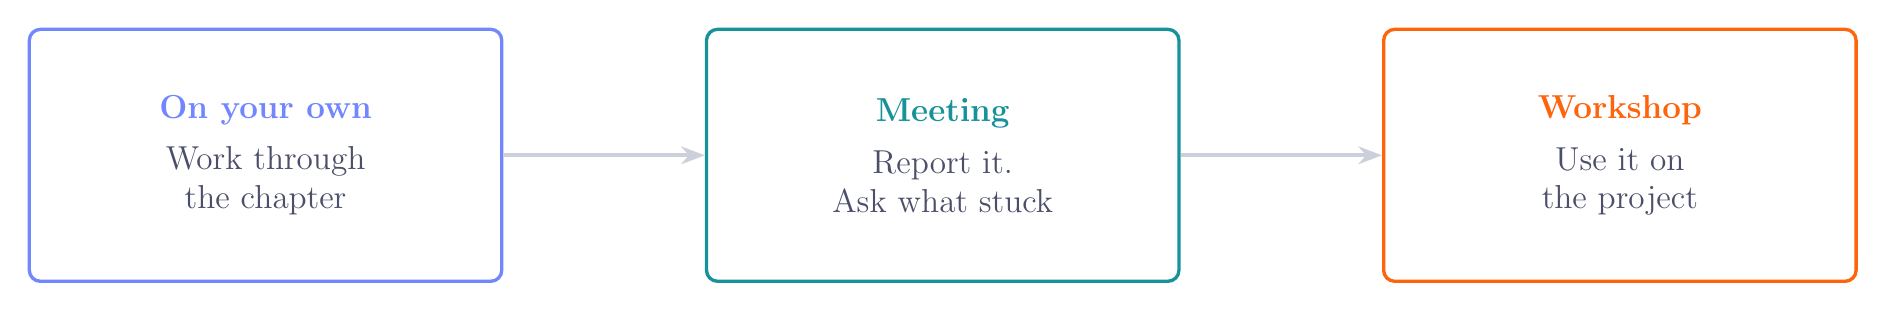
\begin{tikzpicture}
  \node[draw=inkblue, line width=1.2pt, rounded corners=4pt, fill=white,
        minimum width=6.0cm, minimum height=3.2cm, align=center,
        font=\large, text=inktext] (read)
    {\textbf{\color{inkblue} On your own}\\[0.4em] Work through\\ the chapter};
  \node[draw=inkteal, line width=1.2pt, rounded corners=4pt, fill=white,
        minimum width=6.0cm, minimum height=3.2cm, align=center,
        font=\large, text=inktext] (meet) at (8.6,0)
    {\textbf{\color{inkteal} Meeting}\\[0.4em] Report it.\\ Ask what stuck};
  \node[draw=inkred, line width=1.2pt, rounded corners=4pt, fill=white,
        minimum width=6.0cm, minimum height=3.2cm, align=center,
        font=\large, text=inktext] (work) at (17.2,0)
    {\textbf{\color{inkred} Workshop}\\[0.4em] Use it on\\ the project};
  \draw[-{Stealth[length=3mm]}, inkfaint, line width=1.4pt] (read) -- (meet);
  \draw[-{Stealth[length=3mm]}, inkfaint, line width=1.4pt] (meet) -- (work);
\end{tikzpicture}
\end{center}

\vspace{1.0cm}

\begin{center}
{\LARGE The first box is homework.\\[0.4em]
 The other two are \textbf{timetabled}, every group-project week.}
\end{center}

\vspace{0.5em}

\begin{center}
{\large\color{inkgrey} You do not have to find a free hour between four
diaries. It is on your timetable.}
\end{center}

\newpage
\slidehead{Groups}

\vspace{1.6cm}

\begin{center}
{\LARGE Groups of \textbf{four}, and \textbf{you choose}.}

\vspace{1.6cm}

{\LARGE Not registered by the deadline?}

\vspace{0.7em}

{\LARGE\bfseries\color{inkred} Assigned at random.}
\end{center}

\newpage
\slidehead{This week}

\vspace{0.9cm}

{\LARGE
\textbf{\color{inkblue}1.}\quad Form your group of four and register it.

\vspace{0.9em}

\textbf{\color{inkblue}2.}\quad Read the Assessment page.

\vspace{0.9em}

\textbf{\color{inkblue}3.}\quad Open one worked example project.

\vspace{0.9em}

\textbf{\color{inkteal}4.}\quad \textbf{Email me to talk through a
topic:} \texttt{knightva@cardiff.ac.uk}}

\vspace{1.1cm}

\begin{center}

\begin{tikzpicture}
  \node[draw=inkred, line width=1.4pt, rounded corners=4pt, fill=white,
        minimum width=21cm, minimum height=2.8cm,
        text width=19.8cm, align=center, inner sep=0.4cm,
        text=inktext, font=\large] {%
    \textbf{\color{inkred} Your group meets every group-project week,
    in your own slot.}\\[0.4em]
    Print the week's minutes form, complete it at the meeting, and bring
    it to the next class session. Five forms, and \(I\) is counted from
    them.};
\end{tikzpicture}
\end{center}

\end{document}
